% Vorbereitung: Vorbereitungsaufgaben bearbeiten
% Versuchsaufbau: Verwendete Apparatur, Beschreibung Funktionsweise/Nutzen mit Skizze/Foto
\section{Durchführung}
\label{sec:durchführung}

Im Folgenden wird der Versuchsaufbau erklärt und die Messdurchführung wird beschrieben.

\subsection{Versuchsaufbau}
\label{sec:Versuchsaufbau}
Die \autoref{fig:bild4} zeigt die transparente Grundplatte, welche zur Untersuchung der grundlegende Gesetzmäßigkeiten der Strahlenoptik und der Wellenoptik
verwendet wird.
\begin{figure}[H]
    \centering
	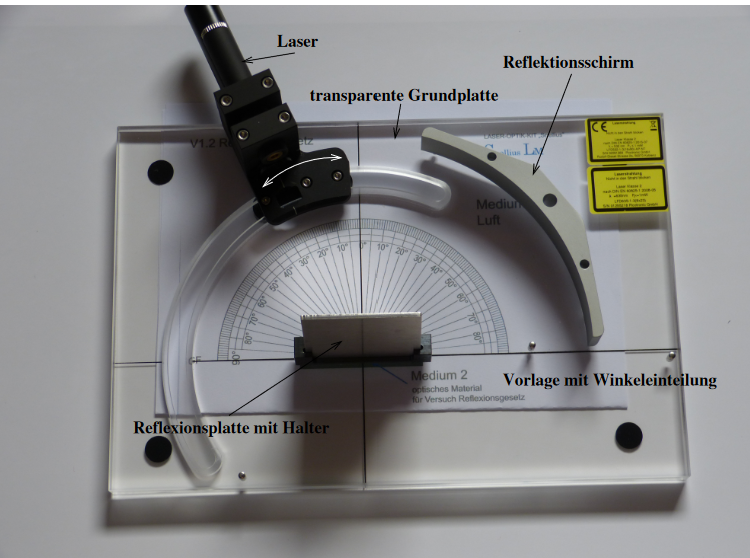
\includegraphics[width=0.6\linewidth]{content/grafik/aufbau.png}
	\caption{Transparente Grundplatte auf der sich zwei Laserdiodenmodule befinden. \cite{reflex}}
	\label{fig:bild4}
\end{figure}
Auf der Platte befinden sich zwei Laserdiodenmodule, welche Licht mit der Wellenlänge $\lambda_{\text{rot}} = \SI{635}{\nano\meter}$ und
$\lambda_{\text{grün}} = \SI{532}{\nano\meter}$ emittieren. Diese Laserdioden lassen sich im Halbkreis bewegen.
In der Mitte  des Halbkreises lassen sich für die unterschiedlichen Versuchsaufgaben verschiedene geometrische Elemente einbauen.

\subsection{Versuchsaufgabe}
\label{sec:Versuchsaufgaben}

Zunächst wird das Reflexionsgestz untersucht, indem der gründe Laser, die Vorlage a und der Halter mit dem Spiegel verwendet werden.
Für 7 Einfallswinkel $\alpha_1$ werden die Ausfallswinkel $\lambda_2$ gemessen.

Als Zweites wird das Brechungsgesetz untersucht, dafür wird der Brechungsindex von Luft $n_1 = 1$ genähert.
Verwendet werden der grüne Laser, die Vorlage a und die planparallele Platte. Die Platte wird so positioniert, dass 
der Eintrittsspalt zur Winkelskala zeigt. Die \autoref{fig:bild5} zeigt den Prozess, bei dem der Lichtstrahl durch eine planparallele
Platte geht und dabei zwei Brechungen erfährt.
\begin{figure}[H]
    \centering
	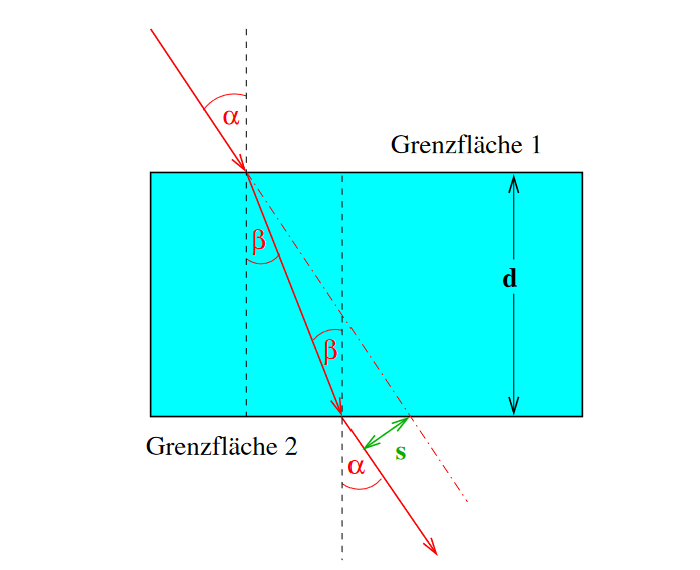
\includegraphics[width=0.6\linewidth]{content/grafik/strahlen.png}
	\caption{Strahlenversatz an einer planparallelen Platte. \cite{reflex}}
	\label{fig:bild5}
\end{figure}
Der Strahlenversatz $s$ lässt sich berechnen über die Gleichung 
\begin{equation}
	s=d \frac{\sin (\alpha-\beta)}{\cos \beta}.
	\end{equation}
Bestimmt wird der Brechungswinkel $\beta$ für 7 verschiedene Einfallswinkel $\alpha$.

Ein optisches Prisma wird durch nicht parallele Flächen begrenzt.